\documentclass[tikz]{standalone}
\usetikzlibrary{shapes.geometric, arrows, backgrounds}


\tikzstyle{dot} = [circle, minimum width=0.5cm, minimum height=0.5cm, text centered, draw=black]
\tikzstyle{arrow} = [thick,->,>=stealth]
\tikzstyle{data} = [ellipse, minimum width=2cm, minimum height=1cm, text centered, draw=black]
\tikzstyle{operation2} = [rectangle, rounded corners, minimum width=2cm, minimum height=1cm, text centered, draw=black]
\tikzstyle{split} = [rectangle, minimum height=2cm, minimum width=1cm, align=center, draw=black]
\tikzstyle{arrow2} = [thick,->,>=stealth,double]

\begin{document}
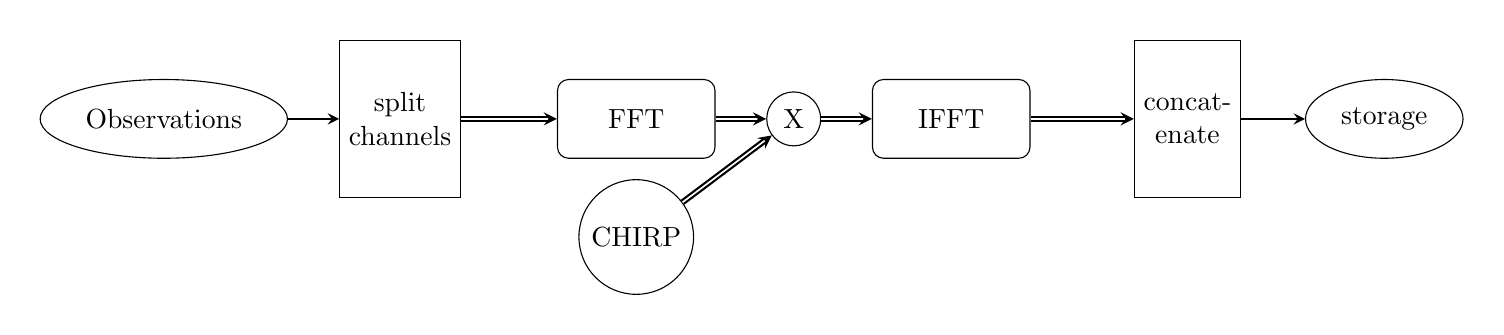
\begin{tikzpicture}[node distance=2cm, background rectangle/.style={fill=white}, show background rectangle]
\node (in) [data] {Observations};
\node (split) [split, right of=in, xshift=1cm] {split\\ channels};
\node (fft) [operation2, right of=split, xshift=1cm] {FFT};
\node (mp) [dot, right of=fft] {X};
\node (ifft) [operation2, right of=mp] {IFFT};
\node (concat) [split, right of=ifft, xshift=1cm] {concat-\\enate};
\node (ram) [data, right of=concat, xshift=0.5cm] {storage};
\node (chirp) [dot, below of=fft, yshift=0.5cm] {CHIRP};

\draw [arrow] (in) -- (split);
\draw [arrow2] (split) -- (fft);
\draw [arrow2] (fft) -- (mp);
\draw [arrow2] (mp) -- (ifft);
\draw [arrow2] (ifft) -- (concat);
\draw [arrow] (concat) -- (ram);
\draw [arrow2] (chirp) -- (mp);
\end{tikzpicture}
\end{document}
